\section{Verifying the model with Parallel DataSeries}
\label{sec:pds}

The Hadoop results above clearly diverge from the predicted optimal.
The large extent to which they diverge, however, brings the accuracy
of the model into question.  To validate our model, we present
Parallel DataSeries (PDS), a data analysis tool that attempts to
closely approach the maximum possible throughput.

\minorsection{PDS Design} Parallel DataSeries builds on DataSeries, an
efficient and flexible data format and runtime library optimized for
analyzing structured data~\cite{dataseries}.  DataSeries files are
stored as a sequence of \emph{extents}, where each extent is a series
of records.  The records themselves are typed, following a schema
defined for each extent.  Data is analyzed at the record level, but
I/O is performed at the much larger extent level.  DataSeries supports
passing records in a pipeline fashion through a series of modules.
PDS extends DataSeries with modules that support parallelism over
multiple cores (intra-node parallelism) and multiple nodes (inter-node
parallelism), to support parallel flows across modules as depicted in
Figure~\ref{fig:pds}.


{
\renewcommand{\baselinestretch}{1.0}
\begin{figure}[t]
\begin{center}

%\resizebox{\columnwidth}{!} {
%   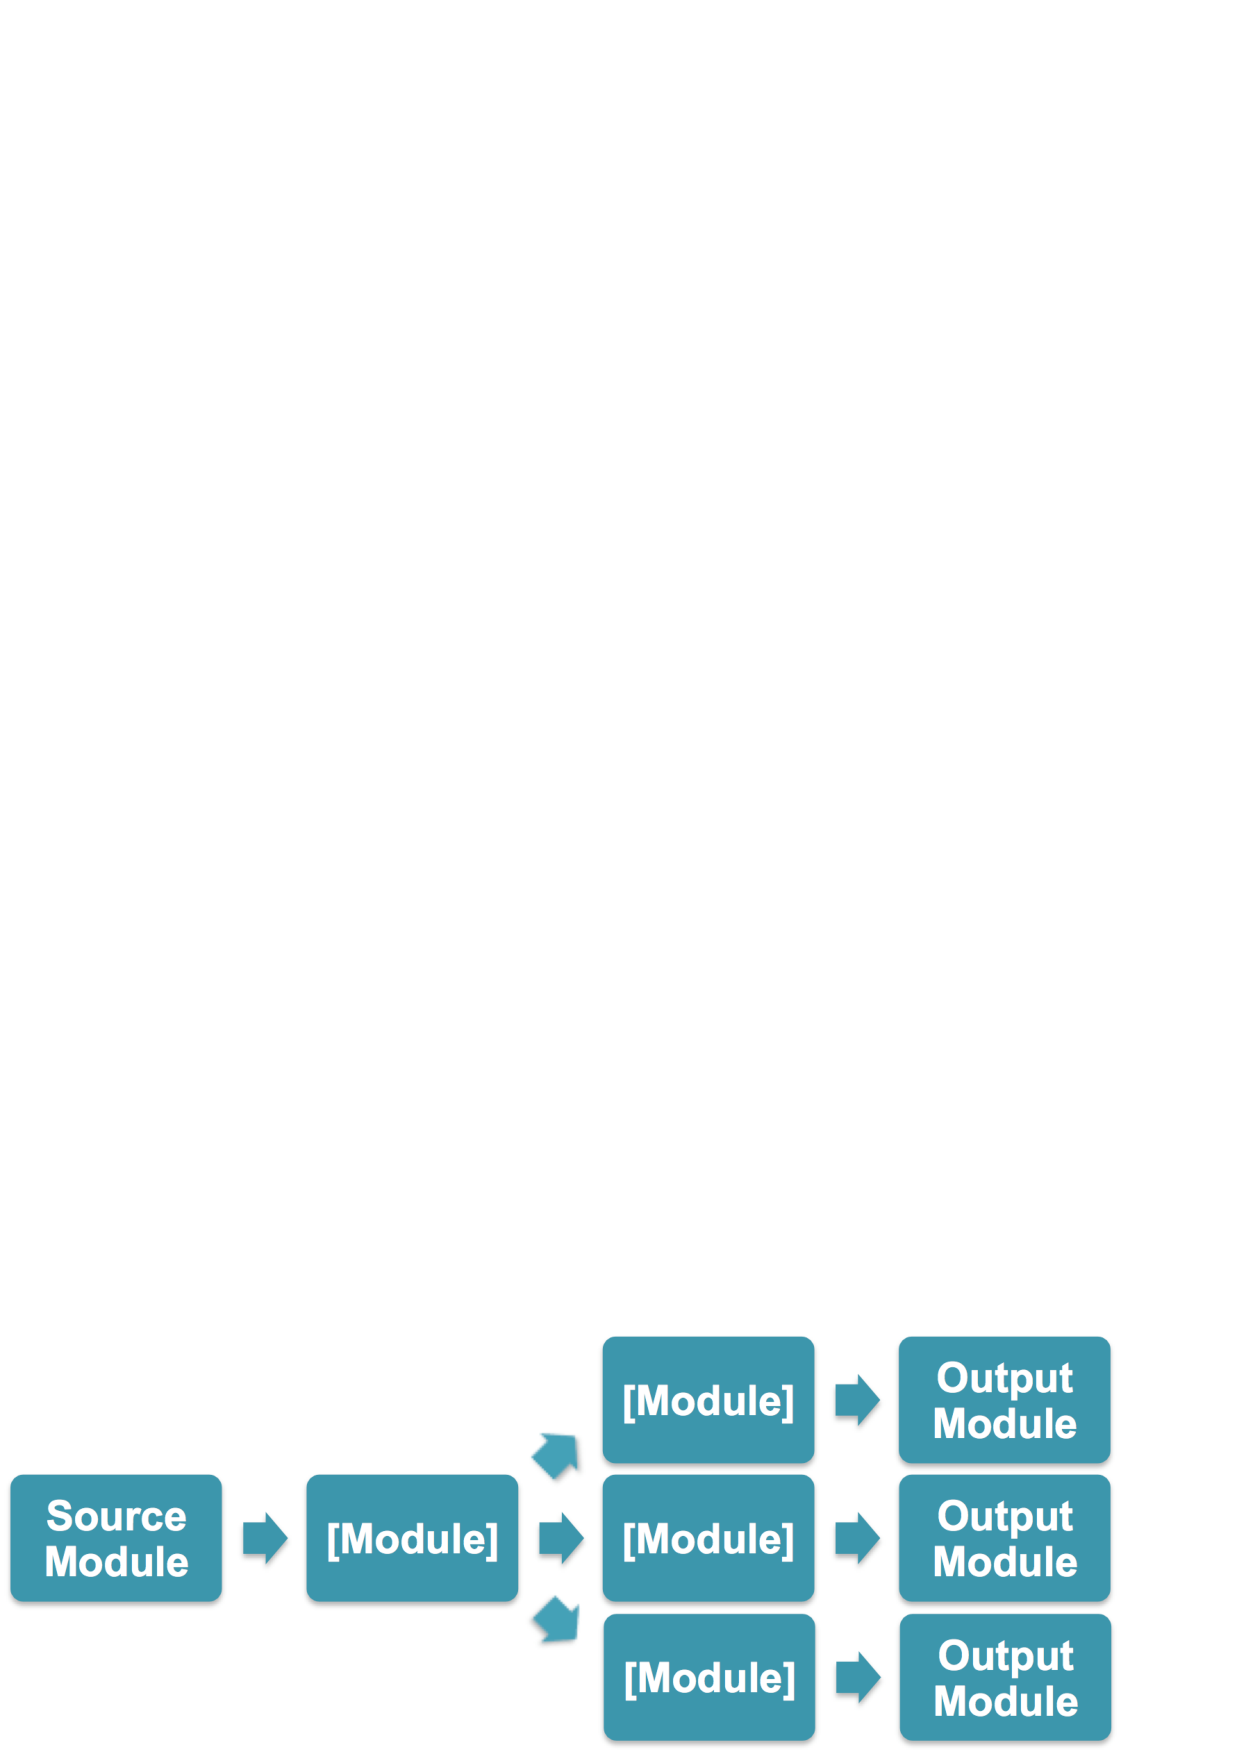
\includegraphics[height=1.5in]{fig_pds.pdf}
   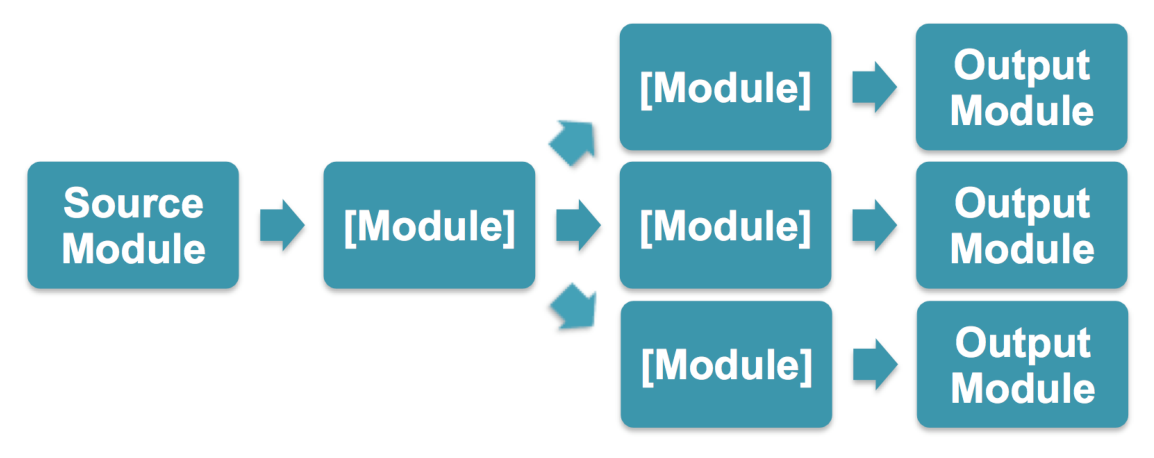
\includegraphics[height=1.5in]{fig_pds.eps}
%}

\end{center}
\minicaption{Parallel DataSeries is a carefully-tuned parallel runtime library for structured data analysis}
{Incoming data is queued and passed in a pipeline through a number of modules in parallel.}

\label{fig:pds}
\end{figure}
}



\minorsection{Sort evaluation} We built a parallel sort module in PDS
that implements a dataflow pattern similar to map-reduce.
In Phase 1, data is
partitioned and shuffled across the network.
As soon as a node receives all data from the shuffle, it exits Phase 1 and
begins Phase 2 with a local sort.  To generate input data for
experiments, we used
\emph{Gensort}, which is the sort benchmark~\cite{sortbenchmark} input generator
on which \emph{TeraGen} is based. The Gensort input set is
separated into partitions, one for each node.
PDS doesn't currently utilize a distributed filesystem, so we
manually partition the input, with 40 million records ($\sim$4 GB) at
each node.  We converted the GenSort data to DataSeries format without
compression, which expands the input by 4\%.
%note the 4 % cannot be from extent headers unless the extents are silly small.
%It is probably alignment overhead in the fixedwidth fields; 2 bytes for the 10 byte
%key (for 12 bytes total) and 2 bytes on the 90 byte record = 4 extra bytes per 100.

We measured PDS to see how closely it performed to the optimal
predicted performance on the same cluster used for the Hadoop
experiments.  Figure~\ref{fig:pds:sort1} presents the equivalent sort task
as run for Hadoop.  We repeated all experiments 10 times, starting
from a cold cache and syncing all data to disk before terminating the
measurement.
%reported, along with error bars for the measured standard deviation in
%each direction.  
As with the earlier Hadoop measurements, time is
broken down into each phase.  Furthermore, average per-node times are
included for the actual sort, as well as a \emph{stragglers} category
that represents the average wait time of a node from the time it
completes all its work until the the last node involved in the
parallel sort also finishes.

PDS performed well at 12-24\% of optimal.  About 4\% of that is the
aforementioned input expansion.  The sort time takes a little over 2
seconds, which accounts for another 3\% of the overhead.  Much of this
CPU could be overlapped with IO (PDS doesn't currently), and it is
sufficiently small to justify excluding CPU time from the model.
These two factors explain most of the 12\% overhead of the single node
case, leaving a small amount of natural coordination and runtime
overhead in the framework.  As the parallel sort is scaled to 25
nodes, besides the additional coordination overhead from code
structures that enable partitioning and parallelism, the remaining
divergence can be mostly explained by two factors: (1) straggler
nodes, and (2) network slowdown effects from many competing transfers.
Stragglers (broken out in Figure~\ref{fig:pds:sort1}b) can be the
result of generally slow (i.e., ``bad'') nodes, skew in network
transfers, or variance in disk write times.  The up to 5\% observed
straggler overhead is reasonable.  The network slowdown effects were
identified in Section~\ref{sec:measure} using \texttt{iperf}
measurements, and are mostly responsible for the slight time increase
starting around 4 nodes.  However, even if the effective network
goodput speeds were 100 MB/s instead of the 110 MB/s used with the
model, that would eliminate only 4\% of the additional overhead for
our PDS results compared to the predicted optimal time.  As more nodes
are added at scale, the straggler effects and network slowdowns become
more pronounced.

{
\renewcommand{\baselinestretch}{1.0}
\begin{figure}[t]
\begin{center}
\subfigure[Scaling a PDS sort benchmark up to 25 nodes.]{
\includegraphics{fig_pds_sort1.eps}
\label{fig:pds:sort1:scale}
}
\subfigure[Time breakdown.]{
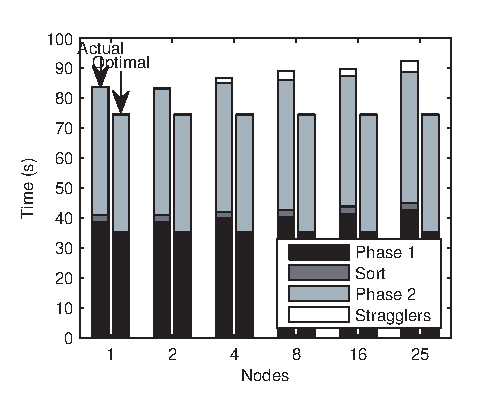
\includegraphics{fig_pds_breakdown1.eps}
\label{fig:pds:sort1:breakdown}
} \minicaption{Using Parallel DataSeries to sort up to 100~GB, it is
  possible to approach within 12-24\% of the optimal sort times as
  predicted by our performance model} {PDS scales well for an
  in-memory sort with 4~GB per node up to 25 nodes in {\bf (a)},
  although there is a small time increase starting around 4 nodes due
  to network effects.  Also shown for the 25 node case is the
  performance of our older, unbalanced partitioner, which had an
  additional 6\% performance overhead from optimal.  A breakdown of
  time in {\bf (b)} shows that the time increases at scale are mostly
  in the first phase of a map-reduce dataflow, which includes the
  network data shuffle, and in the time nodes spend waiting for
  stragglers due to effects of skew. }

\label{fig:pds:sort1}
\end{center}
\end{figure}
}



When we originally ran these experiments and inspected the results of
the 25 node case, we noticed that 6 of the nodes consistently finished
later and were processing about 10\% more work than the other 19.  It
turned out that our data partitioner was using only the first byte of
the key to split up the space into 256 bins, so it partitioned the
data unevenly for clusters that were not a power of 2.  After
designing a fairer partitioner that used more bytes of the key, and
applying it to the 25 node parallel sort, we were able to bring down
the overhead from 30\% to 24\%.

To see how both the model and PDS react to the network as a
bottleneck, we configured our network switches to negotiate 100 Mbps
Ethernet.  Just as the $\frac{n-1}{n} N$ term in the model predicts
increasingly longer sort times which converge in scale as more nodes
participate, Figure~\ref{fig:pds:sort2} demonstrates that our actual
results with PDS match up very well to that pattern.  The PDS sort
results vary between 12-27\% slower than optimal.
%FIXME waiting for new numbers to update this:
%with the same outlier at 25 nodes due to poor partitioning.  
For clusters of size 16 and 25, 5\% of the time is spent waiting for
stragglers. The slow speed of the network amplifies the effects of
skew; we observed a few nodes finishing their second phase before the
most delayed nodes had received all of their data from the first
phase.

{
\renewcommand{\baselinestretch}{1.0}
\begin{figure}[t]
\begin{center}
\subfigure[Scaling a PDS sort benchmark up to 25 nodes.]{
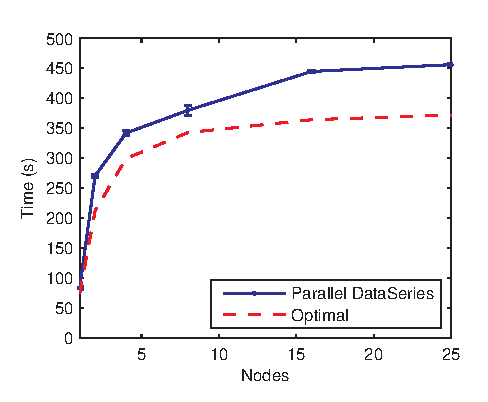
\includegraphics{fig_pds_sort2.eps}
\label{fig:pds:sort2:scale}
}
\subfigure[Time breakdown into phases.]{
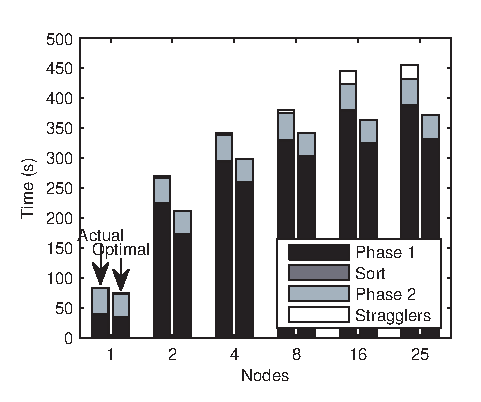
\includegraphics{fig_pds_breakdown2.eps}
\label{fig:pds:sort2:breakdown}
}
\minicaption{With 100~Mbps Ethernet as the bottleneck resource,
  a 100~GB sort benchmark on Parallel DataSeries matches up well with
  the model's prediction and stays within 12-27\% of optimal}
{As more data is sent over the network with larger cluster sizes in
  {\bf (a)}, both the model
  and PDS predict longer sort times that eventually converge.
  A breakdown of time in {\bf (b)} shows that the predicted and actual
  time increases occur during the first map-reduce phase, which
  includes the network data shuffle.}

\label{fig:pds:sort2}
\end{center}
\end{figure}
}


